\documentclass{beamer}
%\documentclass[aspectratio=169]{beamer}
%
\mode<presentation>
{
  \usetheme{default}      
  \usecolortheme{default}
  \usefonttheme{default} 
  \setbeamertemplate{navigation symbols}{}
  \setbeamertemplate{caption}[numbered]
} 

\usepackage[english]{babel}
\usepackage[utf8x]{inputenc}
\usepackage{bbm}

\newcommand{\1}[1]{\mathbbm{1}\left[#1\right]}
\newcommand{\norm}[1]{\left\lVert#1\right\rVert}

\title[Classification]{Introduction to Machine Learning}
\subtitle{Lecture 6: Conclusion}
\author{Alexis Zubiolo\newline\texttt{alexis.zubiolo@gmail.com}}
\institute{Data Science Team Lead @ Adcash}
\date{\today}

\begin{document}

\begin{frame}
  \titlepage
\end{frame}

\begin{frame}{Outline}
This lecture includes:
\begin{itemize}
 \item A \textbf{model selection} lab
 \item A few aspects of machine learning we have not mentioned
 \begin{itemize}
 	\item \textbf{Feature engineering}
 	\item \textbf{Dimensionality reduction}
 \end{itemize}
 \item Feedback and final Q\&A
\end{itemize}
\end{frame}


\begin{frame}
\begin{center}
\Huge{Dimensionality reduction}
\end{center}
\end{frame}

\begin{frame}{Dimensionality reduction}
When working on real-world data sets, the data is not always clean and ready to use.
\vfill
\pause
For example, in some data sets, one may encounter the following issues:
\begin{itemize}
	\item There are too many samples
	\item There are too many features
	\item Some of the features bring no information
\end{itemize}
\vfill
\pause
Hence, there is a need to pre-process the data.
\end{frame}

\begin{frame}{Dimensionality reduction}
In case there are too many samples, a simple solution is to apply subsampling, \textit{e.g.} just take into account 10\% of the samples.
\begin{itemize}
	\item Recall the mini-batch $k$-means
	\item Be careful with the \textbf{class balance}
	\begin{itemize}
		\item Imbalanced classes: \textbf{subsample the majority class}
		\item Little to no imbalance: \textbf{Stratified sampling}
	\end{itemize}
\end{itemize}
\vfill
\pause
It is also important to use common sense and expert knowledge when possible:
\begin{itemize}
	\item Some variables might be intuitively meaningless to solve the ML problem
	\item 
\end{itemize}
\end{frame}

\begin{frame}{Dimensionality reduction with PCA}
PCA = Principal Component Analysis
\vfill
\pause
Rough idea:
\begin{itemize}
	\item Find high variance axes
	\item Select the $k$ axes with the highest variances
	\item Project the data on these axes
\end{itemize}
\vfill
\pause
\begin{figure}
\centering
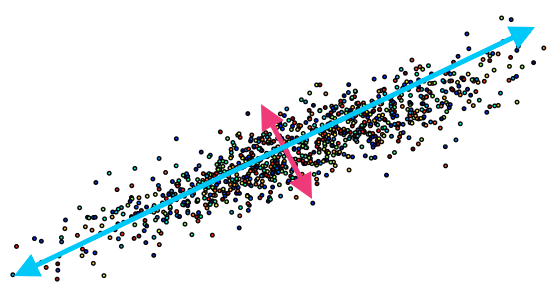
\includegraphics[width=\textwidth]{images/pca_illustration.png}
\end{figure}
\end{frame}

\begin{frame}
\begin{center}
\Huge{Feature engineering}
\end{center}
\end{frame}

\begin{frame}{Feature engineering}
Feature engineering is a key component of machine learning.
\vfill
\pause
Sometimes, on the same data, most algorithm would give roughly the same accuracy (or any other metric). In this case, feature engineering could be the best solution to improve classification/regression results.
\vfill
\pause 
Feature engineering is often \textbf{data-dependent}: You won't use the same features from text data and from images or videos.
\end{frame}

\begin{frame}{Feature engineering in text analysis: TF-IDF}
There are several challenges when dealing with text data:
\begin{itemize}
	\item Mining text can lead to a huge amount of data to process
	\item Not all the data is relevant 
	\item Texts can be of different size
	\item \ldots
\end{itemize}
\pause
\vfill
Hence, there is \textbf{a need to preprocess} it before giving it to any ML algorithm.
\end{frame}

\begin{frame}{Feature analysis in image processing}
In images, we often want to detect interest points such as \textbf{edges} and \textbf{corners}.
\vfill
\pause
SIFT = Scale-Invariant Feature Transform. Invariant to:
\begin{itemize}
	\item Rotation
	\item Difference scales
	\item Affine transformation
	\item (Affine) intensity change
\end{itemize}
\vfill
\pause
\textbf{SIFT is patented} and cannot be used in all situations: There exist alternatives based on the same idea such as SURF (Speeded-Up Robust Features)
\end{frame}

\begin{frame}{SIFT algorithm}
Key steps:
\begin{itemize}
	\item Detect extrema at different scale by difference of gaussians
	\item Detect interest points in the image
	\item Assign orientations to create SIFT features
\end{itemize}
\end{frame}

\begin{frame}{SIFT: Difference of Gaussians (DoG)}

\begin{figure}
\centering
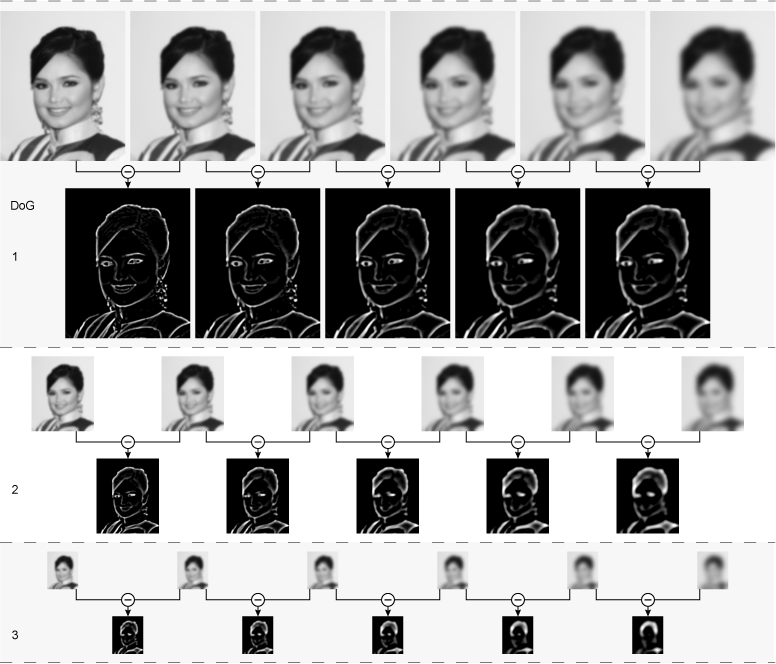
\includegraphics[width=0.75\textwidth]{images/dog.png}
\end{figure}
\end{frame}

\begin{frame}{SIFT: Extrema detection}
Interest points are among the local extrema in the $3\times3\times3$ neighborhood:
\begin{figure}
\centering
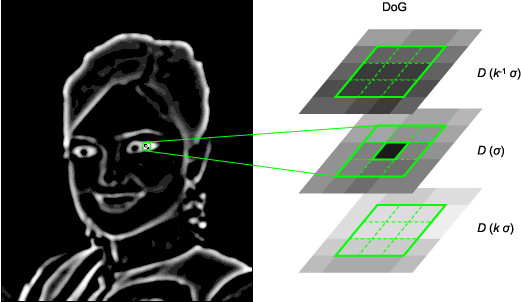
\includegraphics[width=0.75\textwidth]{images/sift_extrema.png}
\end{figure}
\end{frame}

\begin{frame}{SIFT: Extrema detection}
Post-processing:
\begin{itemize}
	\item Remove low-contrast points
	\item Remove points on the edges
\end{itemize}
\pause
\vfill
Before/after:
\begin{figure}
\centering
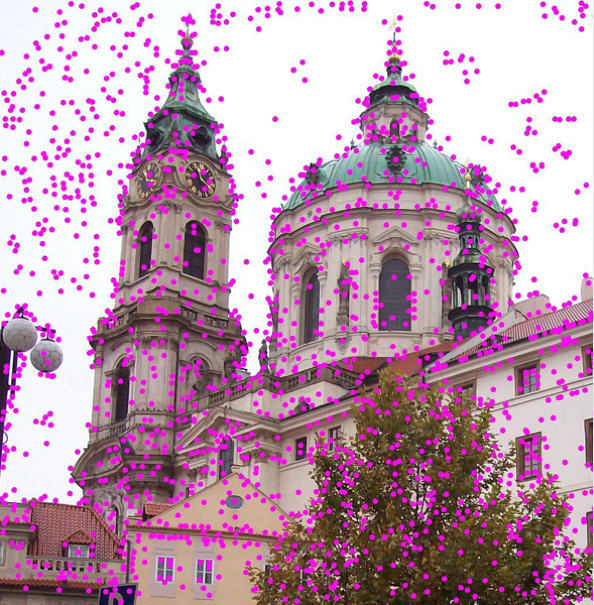
\includegraphics[width=0.5\textwidth]{images/sift_all_points.png}~
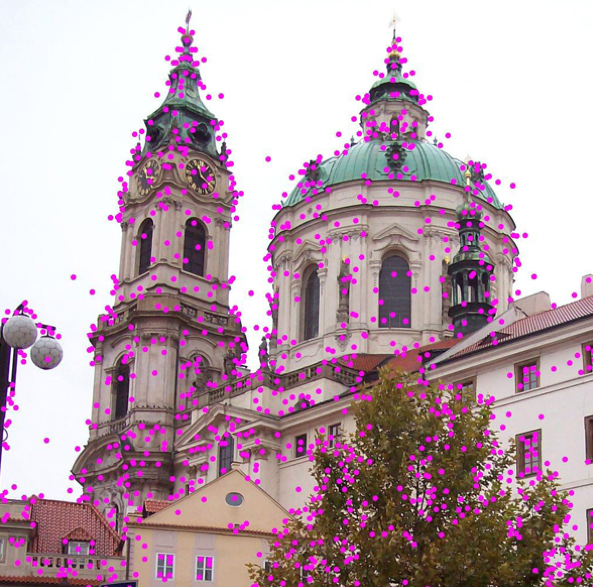
\includegraphics[width=0.5\textwidth]{images/sift_interest_points.png}
\end{figure}
\end{frame}

\begin{frame}{SIFT: Orientation assignment}
For each interest point, compute the orientation histogram:
\begin{figure}
\centering
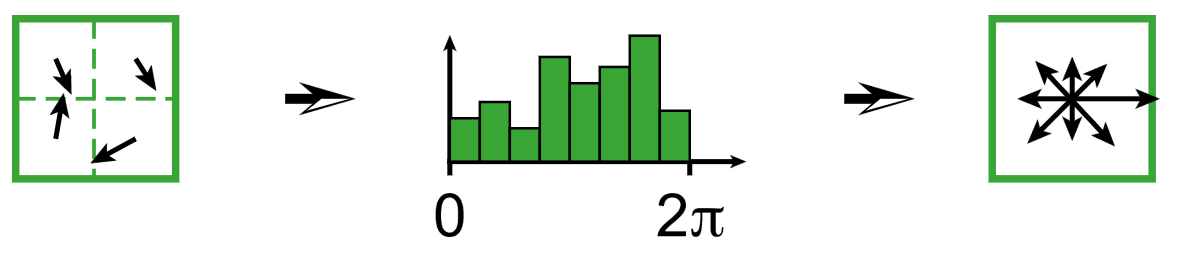
\includegraphics[width=0.75\textwidth]{images/sift_histogram.png}
\end{figure}
Do it for a neighborhood of the interest point:
\begin{figure}
\centering
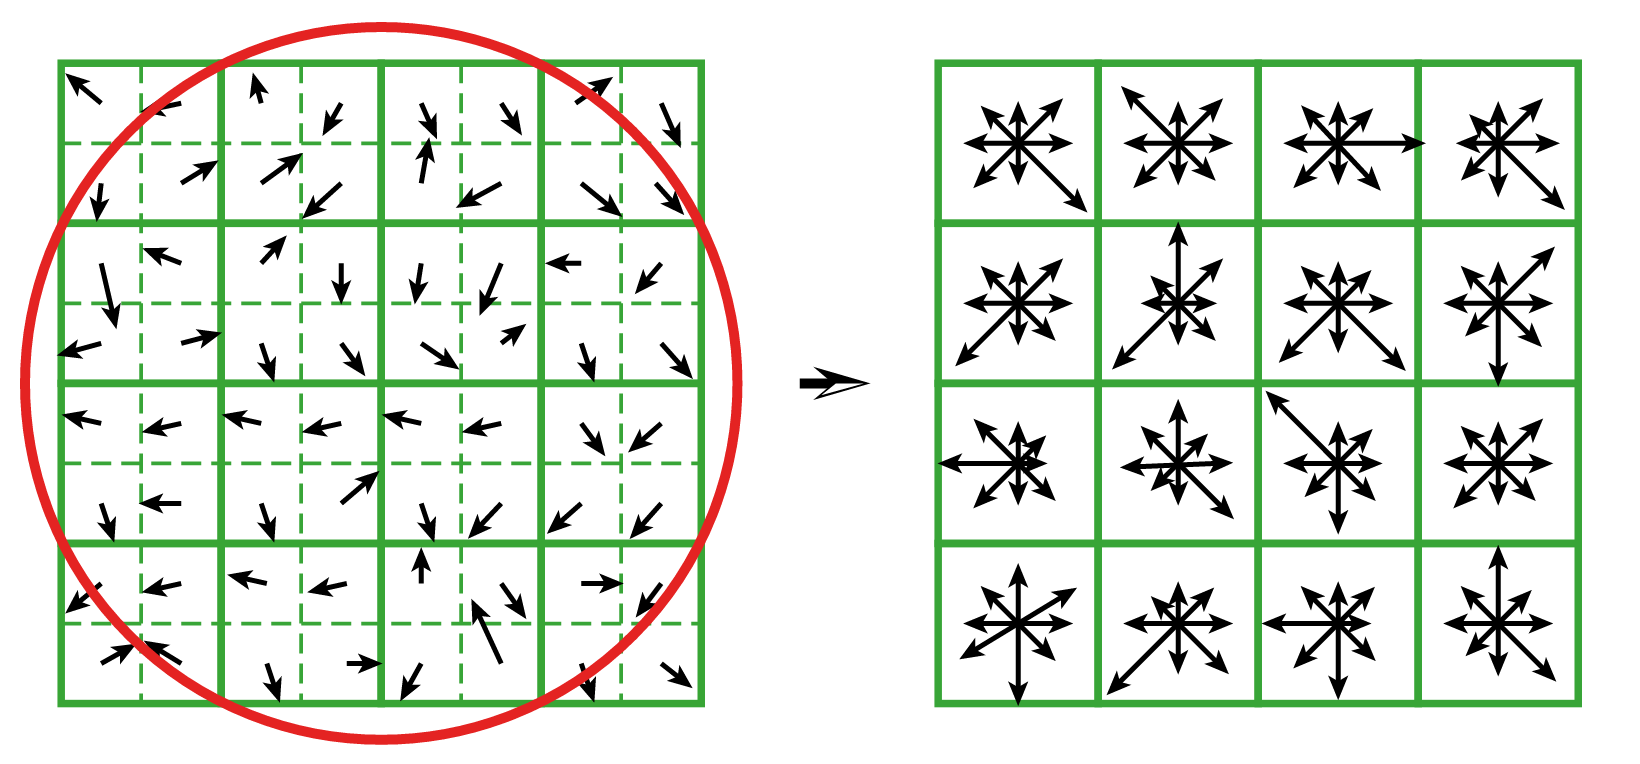
\includegraphics[width=0.75\textwidth]{images/sift_features.png}
\end{figure}
\end{frame}

\begin{frame}{SIFT applications}
SIFT has other applications, such as aligning images, creating panoramas, video tracking, \ldots
\pause
\vfill
YouTube video example
\pause
\vfill
\begin{figure}
\centering
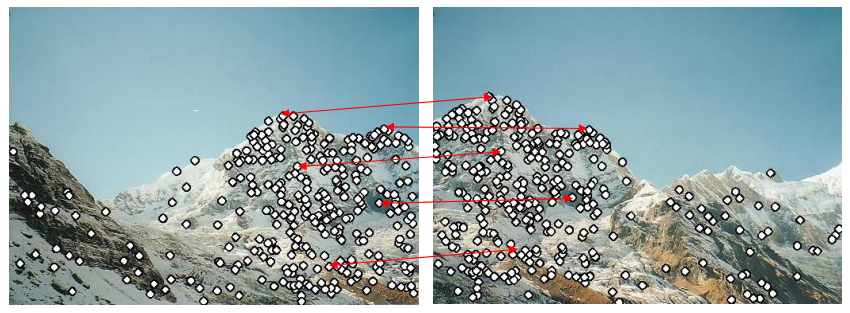
\includegraphics[width=\textwidth]{images/sift_panorama_matching.png}
\end{figure}
\end{frame}

\begin{frame}{SIFT illustration: Panorama}

\begin{figure}
\centering
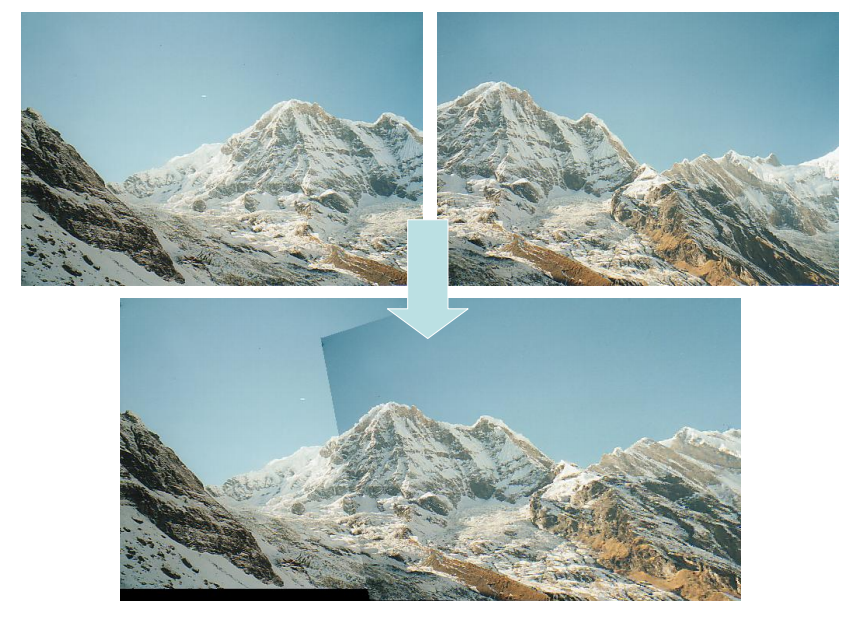
\includegraphics[width=\textwidth]{images/sift_panorama_result.png}
\end{figure}
\end{frame}

\begin{frame}{Conclusion of the conclusion}
ML has plenty of applications as we saw
\pause
\vfill
There's \textbf{no general-purpose solution} (at least for now): It is important to \textbf{look at the data} and \textbf{adapt to the situation}.
\end{frame}

\begin{frame}
\begin{center}
\huge{Thank you! Questions? \\ Any feedback?}
\end{center}
\end{frame}

\end{document}